
\section{Background}
\label{sec:background}

The original data from Beach 6 and Huntington contain different parameters with different pre-processing requirements as described on the \href{https://www.sciencebase.gov/catalog/file/get/5fe22dead34e30b9123f09b5?f=__disk__42%2F04%2F43%2F420443e837a6255bc88b7c942550014ba2c9b1a6&transform=1&allowOpen=true}{website}. To make sure our model aligns with the existing model for a more direct comparison, we decided to operate pre-processing according to the documentation. Below are the attributes of both datasets; pre-processing will be mentioned if it is required and performed by us from the original data.

\subsection{Beach 6}
\begin{enumerate}
    \item ECOLI\_LOG10
    \begin{itemize}
        \item Description: concentration of \textit{E. coli} recorded
        \item Already log$_{10}$ transformed
    \end{itemize}
    \item TURB\_NTRU
    \begin{itemize}
        \item Description: turbidity value
        \item Pre-processing: log$_{10}$ transform
    \end{itemize}
    \item RHUM\_PCT
    \begin{itemize}
        \item Description: relative humidity
    \end{itemize}
    \item WTEMP\_CEL
    \begin{itemize}
        \item Description: water temperature in degree Celsius
    \end{itemize}
    \item BIRDS\_NO
    \begin{itemize}
        \item Description: number of birds spotted around and in the bathing area
    \end{itemize}
    \item CHANGELL\_FT
    \begin{itemize}
        \item Description: lake level change for the past 24 hours
    \end{itemize}
    \item AirportWindSpInst\_mph
    \begin{itemize}
        \item Description: wind speed at 8am
    \end{itemize}
    \item AirportRain48W\_in
    \begin{itemize}
        \item Description: cumulative rainfall for the past 48 hours
        \item Pre-processing: square-root transform
    \end{itemize}
\end{enumerate}

\subsection{Huntington}
\begin{enumerate}
    \item EcoliAve\_CFU
    \begin{itemize}
        \item Description: \textit{E. coli} concentration
        \item Pre-processing: log$_{10}$ transform
    \end{itemize}
    \item Lake\_Temp\_C
    \begin{itemize}
        \item Description: lake temperature in degrees Celsius
    \end{itemize}
    \item Lake\_Turb\_NTRU
    \begin{itemize}
        \item Description: turbidity of the water body
        \item Pre-processing: log$_{10}$ transform
    \end{itemize}
    \item WaveHt\_Ft
    \begin{itemize}
        \item Description: wave height at the time the E.coli sample was collected
        \item Pre-processing: square-root transform
    \end{itemize}
    \item LL\_PreDay
    \begin{itemize}
        \item Description: lake level change for the past 24 hours
    \end{itemize}
    \item AirportRain48W\_in
    \begin{itemize}
        \item Description: cumulative rainfall for the past 24 hours
        \item Pre-processing: square-root transform
    \end{itemize}
\end{enumerate}


\subsection{Data Exploration}
Before diving into building our model, we explored the dataset and plotted correlation graphs to understand the relationships between log$_{10}$ \textit{E. coli} concentration and key features. For Beach6, we found that turbidity shows a strong linear association (Figure~\ref{fig:turbecoli}). We also noted that discrete data points, such as airport instantaneous wind speed (AirportWindSpInst\_mph), can introduce step-like patterns that complicate linear fits and their visual interpretation (Figure~\ref{fig:airportwindsp}).


\begin{figure}
    \centering
    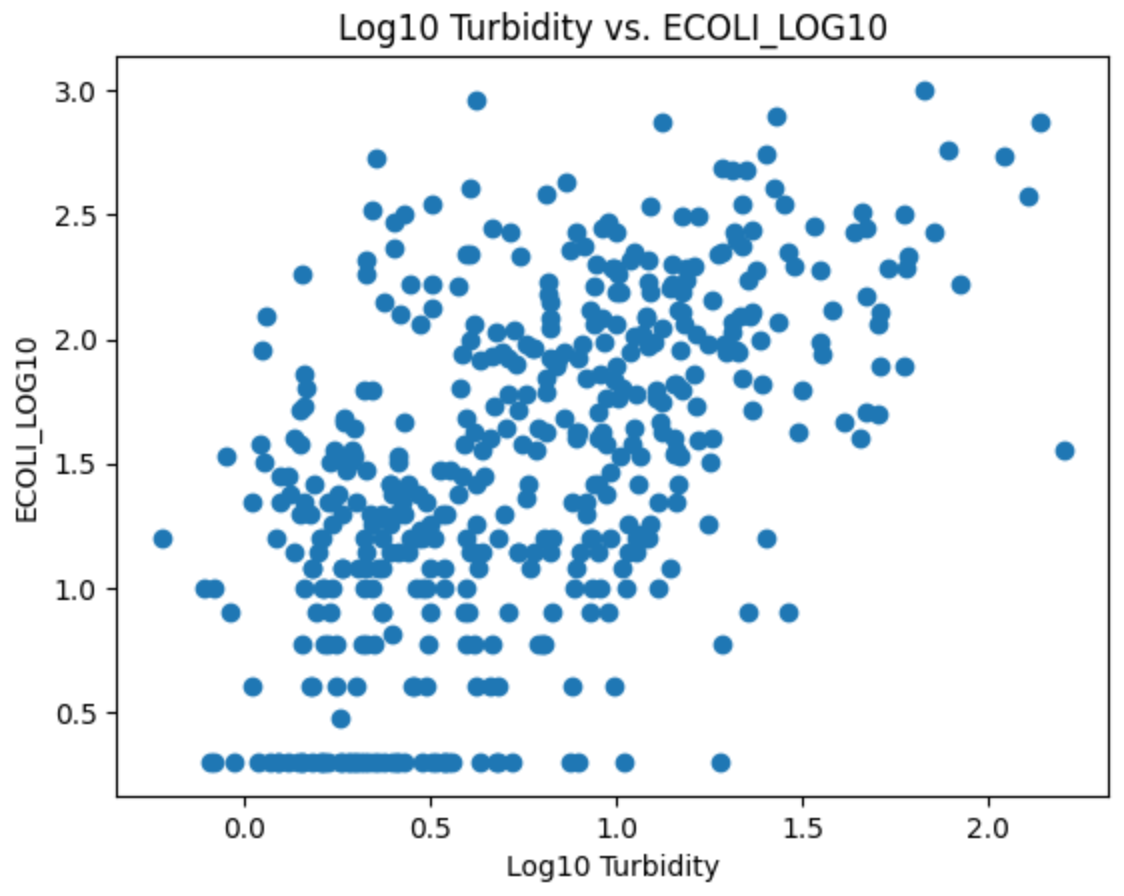
\includegraphics[width=0.47\textwidth]{figs/log10_turb_ecoli.png}
    \caption{Correlation between $\log_{10}$ turbidity and $\log_{10}$ $E. coli$ concentration.}
    \label{fig:turbecoli}
\end{figure}
\begin{figure}
    \centering
    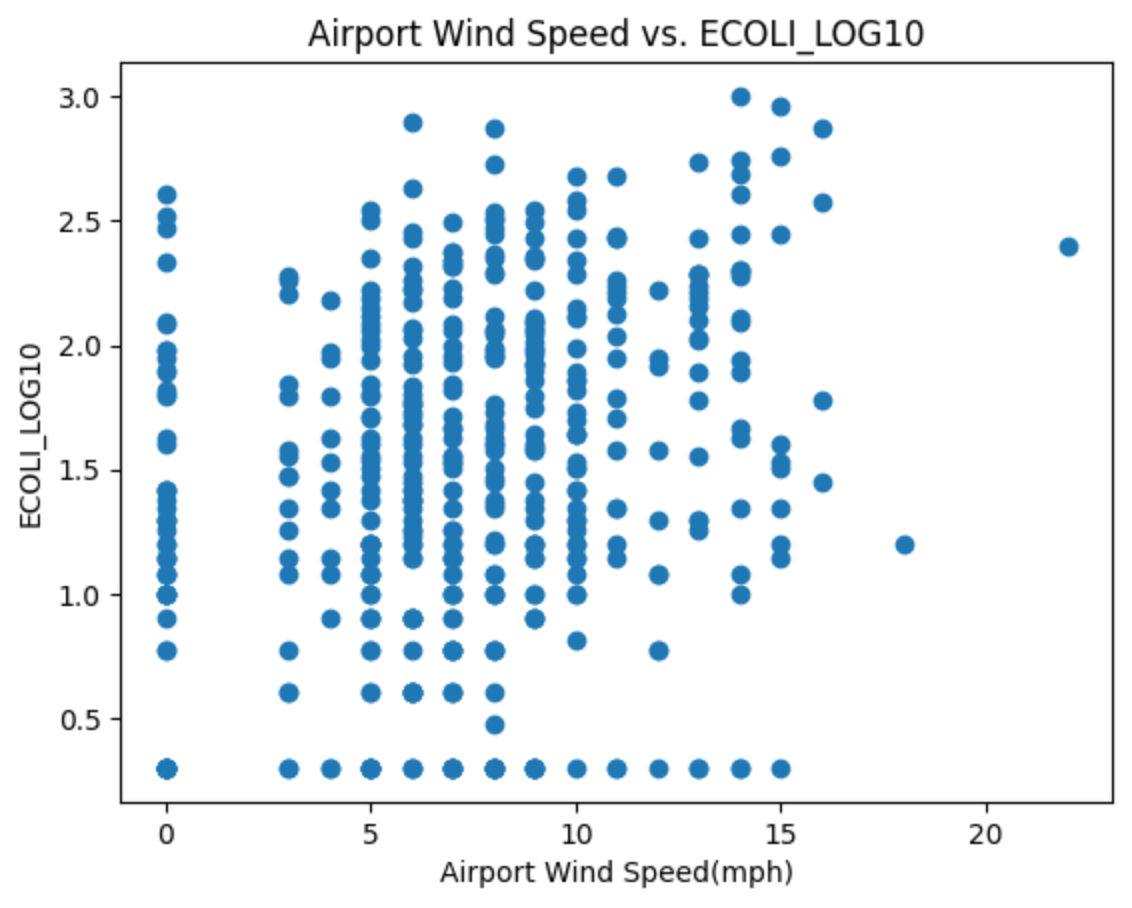
\includegraphics[width=0.47\textwidth]{figs/airportwindsp.png}
    \caption{Correlation between airport wind speed and $\log_{10}$ \textit{E. coli} concentration.}
    \label{fig:airportwindsp}
\end{figure}
